\section{Changing parameter values}
\subsection{Number of Chirps}
    
    \subsubsection*{Parameters}
    \begin{table}[!h]\centering
        \hspace{10mm}
        \begin{tabular}{|l|c|c|}
        \hline
        \multicolumn{1}{|l|}{Parameter} & \multicolumn{1}{l|}{Value} \\
        \hline
        Number of Chirps & 2 \\ 
        \hline
        Chirp Direction & Up \\ 
        \hline
        Carrier Frequency & 2.4G \\ 
        \hline
        IQ rate & 4M \\ 
        \hline
        \end{tabular}
        \caption{Experiment 3-1 parameter values}
    \end{table}
    
    \subsubsection*{Experiment Result}
    \vspace{-4mm}  
    \begin{figure}[!h]\raggedleft
    \hspace{15mm}
		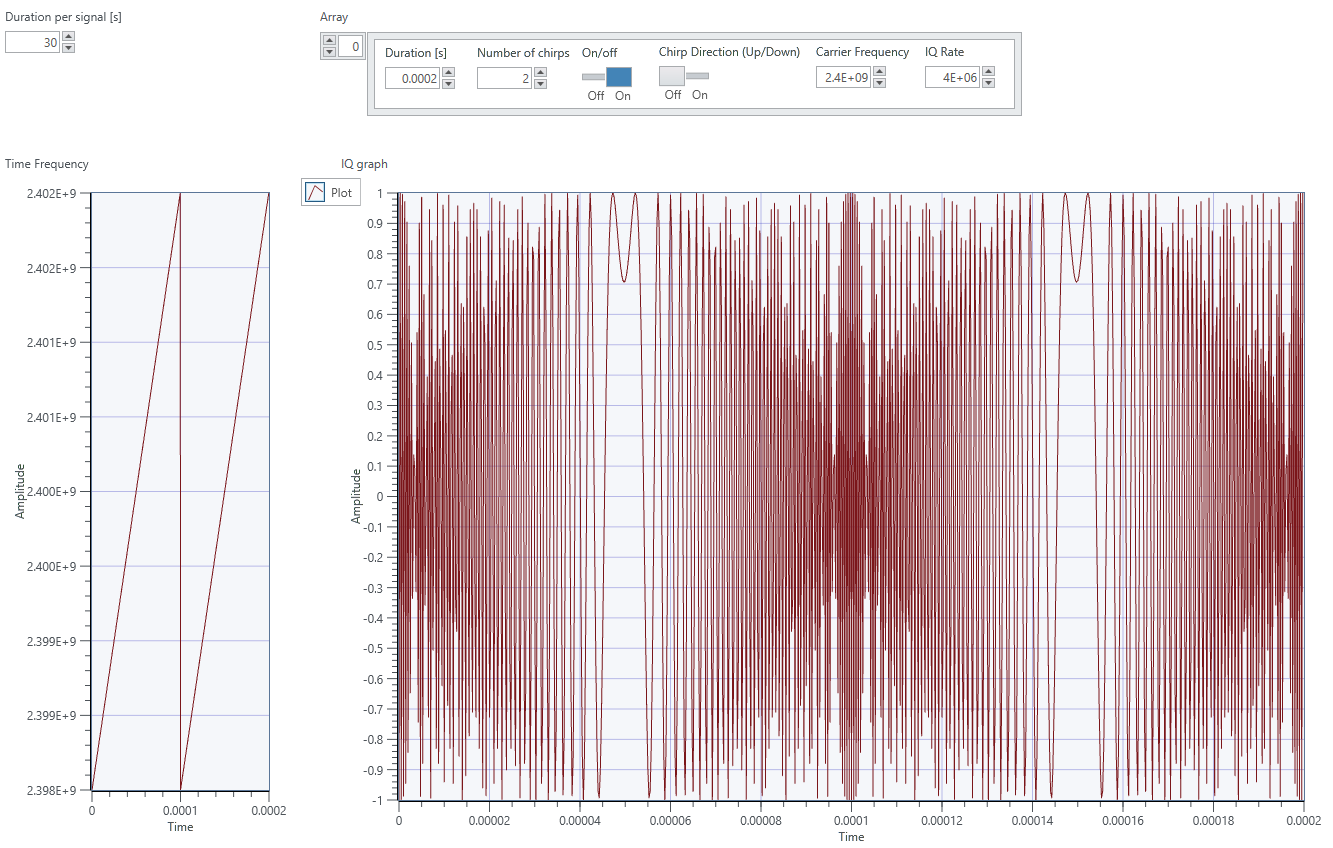
\includegraphics[width=.95\textwidth]{image/week03/3-1-1.png}
		\caption{\footnotesize Experiment 3-1 result}
		\vspace{-10pt}
    \end{figure}
    
    \subsubsection*{Discussion}
    Compared to example of Experiment 2, we changed the number of chirps from 4 to 2. A chirp is a signal that the frequency increases or decreases with time. As we can see in both Time-Frequency graph and IQ graph, the number of chirps changed from 4 to 2. \\
\clearpage    

    %%%%%%%%%%%%%%%%%%%%%%%%%%%%%%%%%%%%%%%%%%%%%%%%%
    
\subsection{Chirps Direction}
    \subsubsection*{Parameters}
    \begin{table}[!h]\centering
        \hspace{10mm}
        \begin{tabular}{|l|c|c|}
        \hline
        \multicolumn{1}{|l|}{Parameter} & \multicolumn{1}{l|}{Value} \\
        \hline
        Number of Chirps & 4 \\ 
        \hline
        Chirp Direction & Down \\ 
        \hline
        Carrier Frequency & 2.4G \\ 
        \hline
        IQ rate & 4M \\ 
        \hline
        \end{tabular}
        \caption{Experiment 3-2 parameter values}
    \end{table}
    
    \subsubsection*{Experiment Result}
    \vspace{-4mm}  
    \begin{figure}[!h]\raggedleft
    \hspace{15mm}
		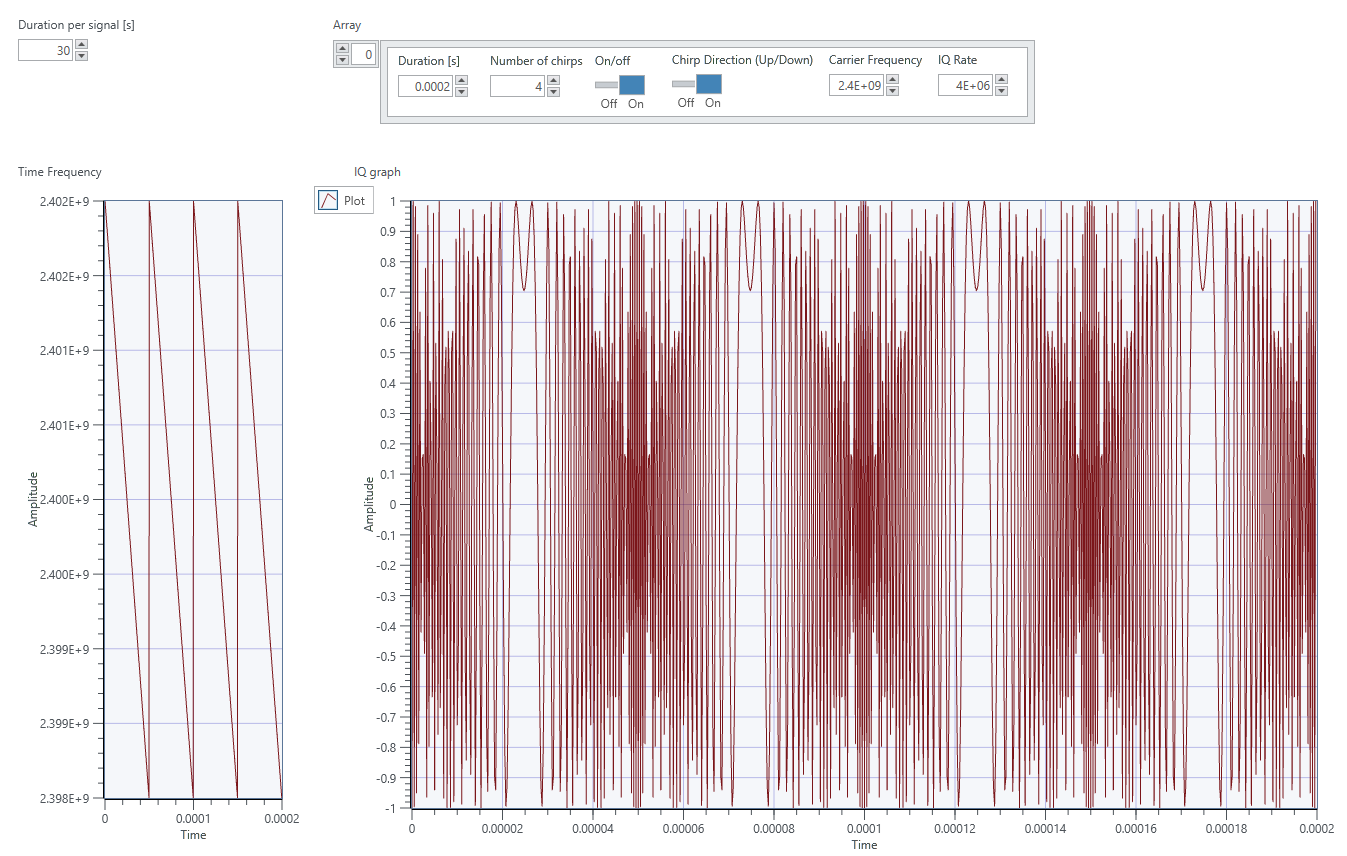
\includegraphics[width=.95\textwidth]{image/week03/3-2-1.png}
		\caption{\footnotesize Experiment 3-2 result}
		\vspace{-10pt}
    \end{figure}
    
    \subsubsection*{Discussion}
    Compared to example of Experiment 2, we changed the chirp direction from ‘Up’ to ‘Down’. As we can see in Time-Frequency graph, the frequency of chirps is increasing linearly in Experiment 2, but it is decreasing linearly in this experiment. However, IQ graphs are the same. \\
\clearpage
    %%%%%%%%%%%%%%%%%%%%%%%%%%%%%%%%%%%%%%%%%%%%%%%%%
    
\subsection{Carrier Frequency : $f = 3.9GHz$}
    \subsubsection*{Parameters}
    \begin{table}[!h]\centering
        \hspace{10mm}
        \begin{tabular}{|l|c|c|}
        \hline
        \multicolumn{1}{|l|}{Parameter} & \multicolumn{1}{l|}{Value} \\
        \hline
        Number of Chirps & 4 \\ 
        \hline
        Chirp Direction & Up \\ 
        \hline
        Carrier Frequency & 2.39G \\ 
        \hline
        IQ rate & 4M \\ 
        \hline
        \end{tabular}
        \caption{Experiment 3-3-1 parameter values}
    \end{table}
    
    \subsubsection*{Experiment Result}
    \vspace{-4mm}  
    \begin{figure}[!h]\raggedleft
    \hspace{15mm}
		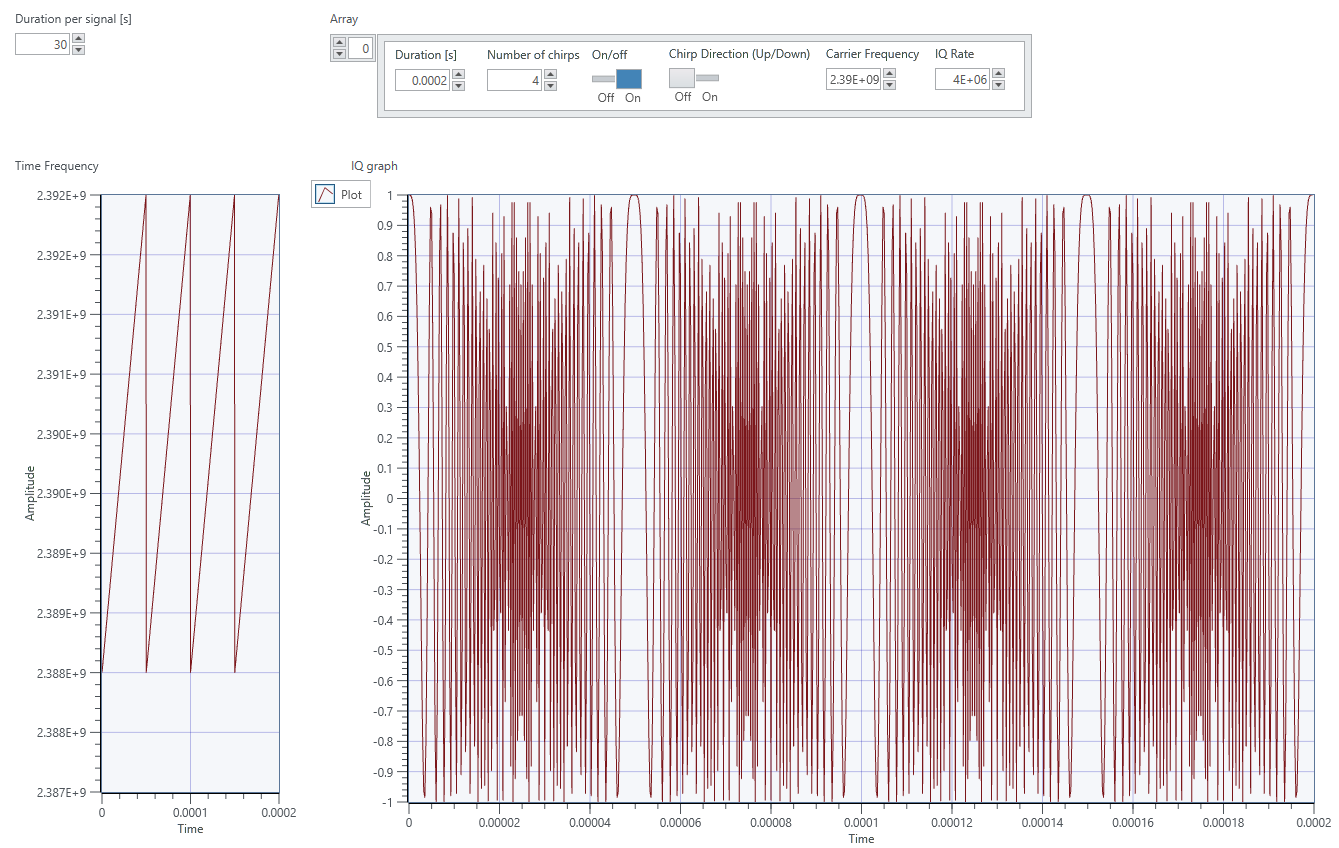
\includegraphics[width=.95\textwidth]{image/week03/3-3-1.png}
		\caption{\footnotesize Experiment 3-3-1 result}
		\vspace{-10pt}
    \end{figure}
\subsection{Carrier Frequency : $f = 4.1GHz$}
    \subsubsection*{Parameters}
    \begin{table}[!h]\centering
        \hspace{10mm}
        \begin{tabular}{|l|c|c|}
        \hline
        \multicolumn{1}{|l|}{Parameter} & \multicolumn{1}{l|}{Value} \\
        \hline
        Number of Chirps & 4 \\ 
        \hline
        Chirp Direction & Up \\ 
        \hline
        Carrier Frequency & 2.41G \\ 
        \hline
        IQ rate & 4M \\ 
        \hline
        \end{tabular}
        \caption{Experiment 3-3-2 parameter values}
    \end{table}
\clearpage
    \subsubsection*{Experiment Result}
    \vspace{-4mm}  
    \begin{figure}[!h]\raggedleft
    \hspace{15mm}
		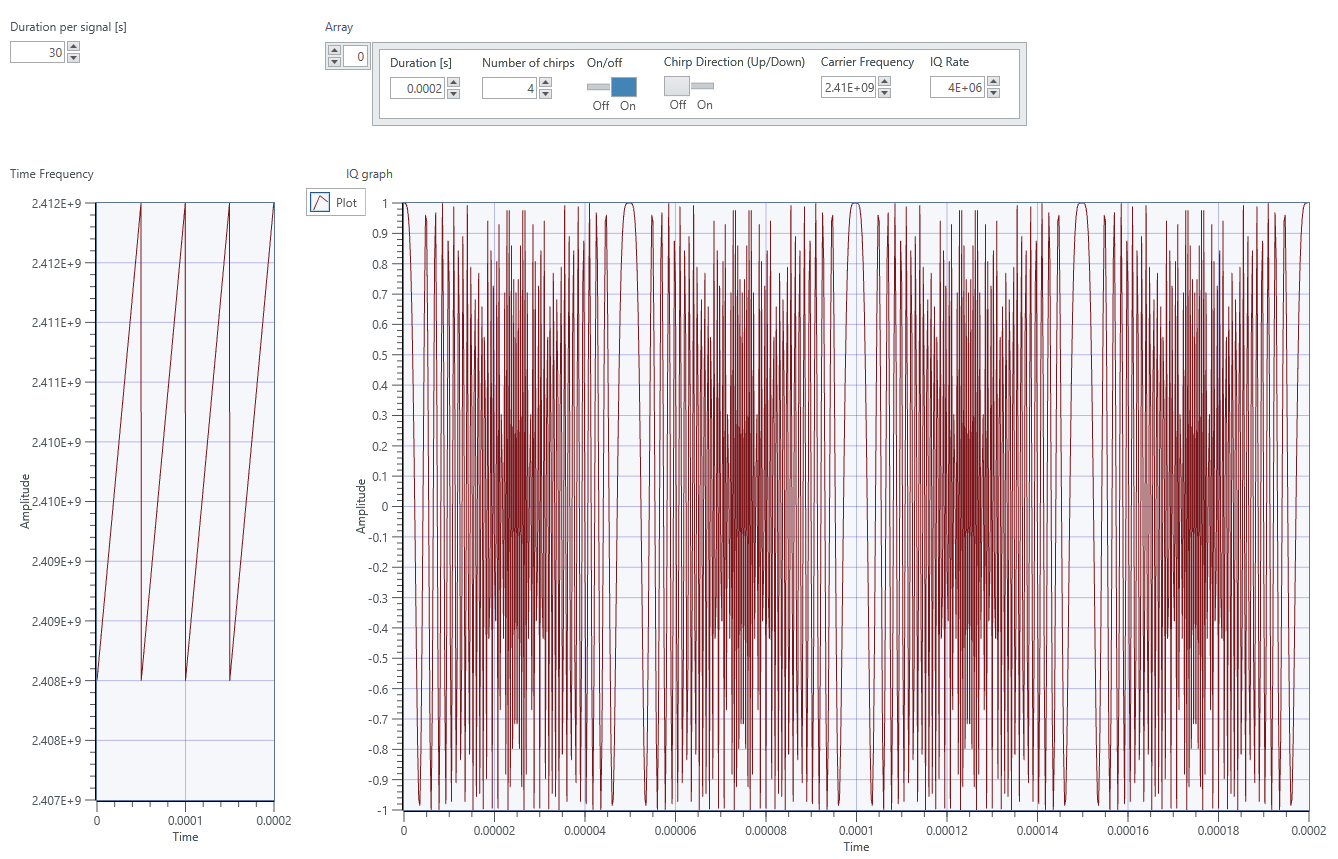
\includegraphics[width=.95\textwidth]{image/week03/3-3-2.png}
		\caption{\footnotesize Experiment 3-3-2 result}
		\vspace{-10pt}
    \end{figure}
    
    \subsubsection*{Discussion with carrier frequency change}
    Compared to example of Experiment 2, we changed the carrier frequency from 2.4G to 2.39G and 2.41G. As we can see in Time-Frequency graph, the carrier frequency is located in the center of the chirp’s frequency range. So, the chirp’s frequency range shifts as the carrier frequency changes. Since the frequency difference is too small, we can’t find difference between IQ graphs. \\
\clearpage
    %%%%%%%%%%%%%%%%%%%%%%%%%%%%%%%%%%%%%%%%%%%%%%%%% 
\subsection{IQ rate (bandwidth) : 8M}
    \subsubsection*{Parameters}
    \begin{table}[!h]\centering
        \hspace{10mm}
        \begin{tabular}{|l|c|c|}
        \hline
        \multicolumn{1}{|l|}{Parameter} & \multicolumn{1}{l|}{Value} \\
        \hline
        Number of Chirps & 4 \\ 
        \hline
        Chirp Direction & Up \\ 
        \hline
        Carrier Frequency & 2.4G \\ 
        \hline
        IQ rate & 8M \\ 
        \hline
        \end{tabular}
        \caption{Experiment 3-4-1 parameter values}
    \end{table}
    \subsubsection*{Experiment Result}
    \vspace{-4mm}  
    \begin{figure}[!h]\raggedleft
    \hspace{15mm}
		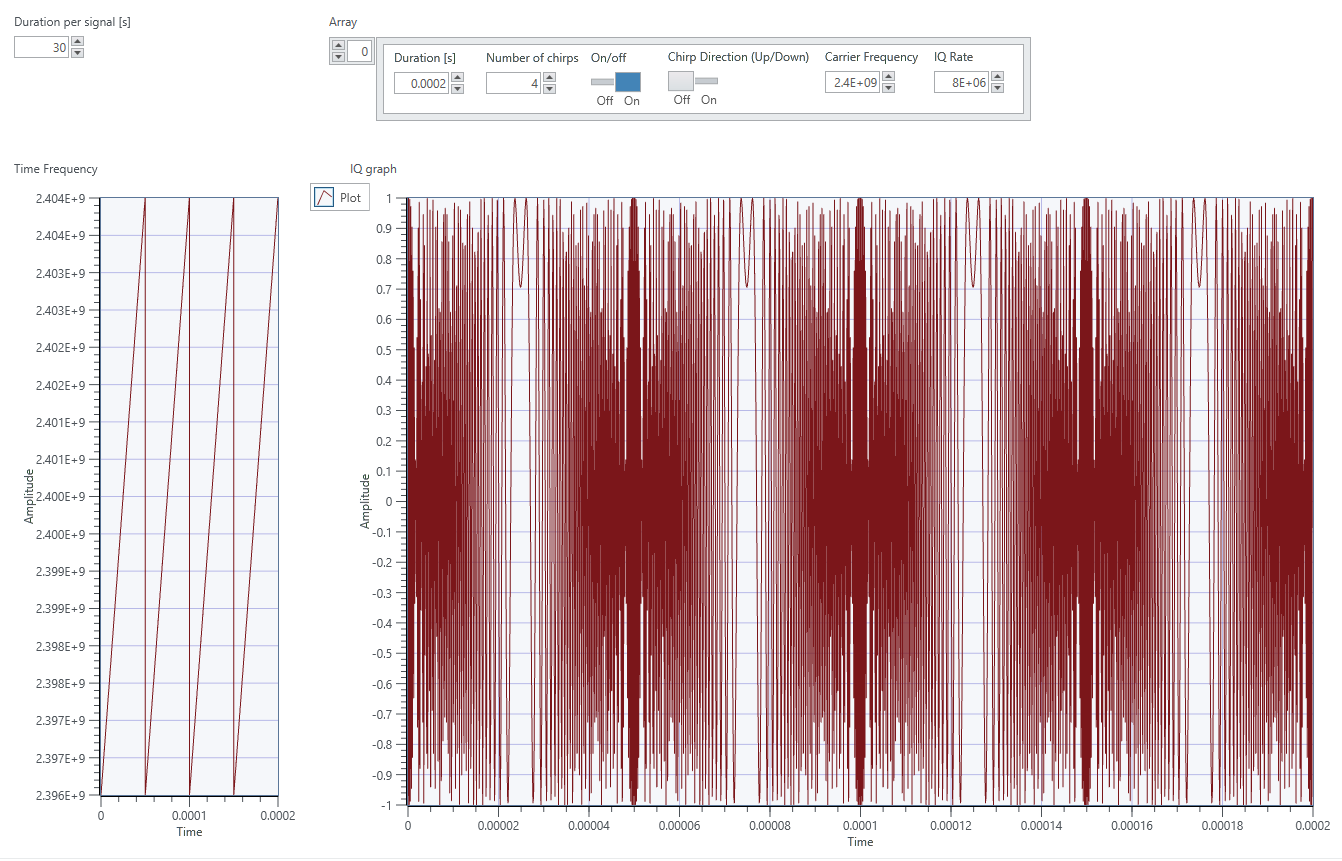
\includegraphics[width=.95\textwidth]{image/week03/3-4-1.png}
		\caption{\footnotesize Experiment 3-4-1 result}
		\vspace{-10pt}
    \end{figure}
\subsection{IQ rate (bandwidth) : 12M}
    \subsubsection*{Parameters}
    \begin{table}[!h]\centering
        \hspace{10mm}
        \begin{tabular}{|l|c|c|}
        \hline
        \multicolumn{1}{|l|}{Parameter} & \multicolumn{1}{l|}{Value} \\
        \hline
        Number of Chirps & 4 \\ 
        \hline
        Chirp Direction & Up \\ 
        \hline
        Carrier Frequency & 2.4G \\ 
        \hline
        IQ rate & 12M \\ 
        \hline
        \end{tabular}
        \caption{Experiment 3-4-2 parameter values}
    \end{table}
\clearpage
    \subsubsection*{Experiment Result}
    \vspace{-4mm}  
    \begin{figure}[!h]\raggedleft
    \hspace{15mm}
		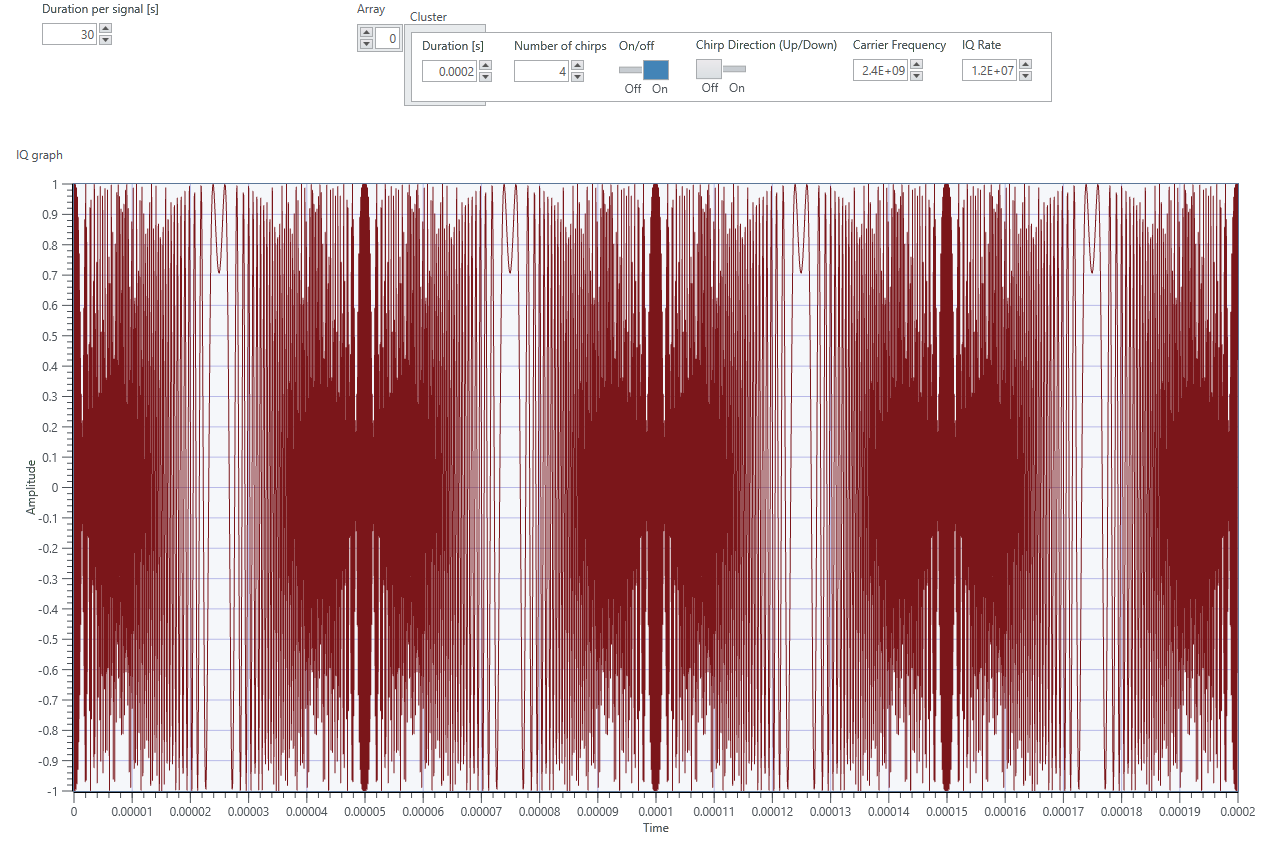
\includegraphics[width=.95\textwidth]{image/week03/3-4-2.png}
		\caption{\footnotesize Experiment 3-4-2 result}
		\vspace{-10pt}
    \end{figure}
    
    \subsubsection*{Discussion}
    Compared to example of Experiment 2, we changed the IQ rate from 4M to 8M and 12M. As we can see in Time-Frequency graph, the IQ rate is equal to chirp’s bandwidth. So, the chirp’s bandwidth increases as the IQ rate increases. Also, IQ graph is denser on time axis as the IQ rate increases. \\
\clearpage